\documentclass[aps,showpacs,twocolumn,floatfix,prx,superscriptaddress]{revtex4-1}
\usepackage{graphicx}
\usepackage{amsfonts}
\usepackage{amsmath}
\usepackage{amssymb}
\usepackage{upgreek}
\usepackage[usenames,dvipsnames]{color}

\begin{document}

\title{Dynamics of 1D polymer maps to ASEP}

\author{Wenwen Huang}
\author{Yen Ting Lin}
\author{Daniela Fr\"{o}mberg}
\author{Jaeoh Shin}
\author{Frank J\"{u}licher}
\author{Vasily Zaburdaev}
\affiliation{Max Planck Institute for the Physics of Complex Systems,
    N\"{o}thnitzer Str. 38, D-01187 Dresden, Germany}

\begin{abstract}
    { abstract text }
\end{abstract}
\maketitle


\section{Introduction}
Many biological processes can be characterized by idealized physical models and
quantitatively studied through the law of physics and methods of
mathematics\cite{Vogel2009,Ding2004,Chou2011,Giorgetti2014,Halverson2014}.  A
good example is the movement of DNA. Polymer models, constructed by bead and rod
or spring, are often utilized to describe
DNA\cite{Giorgetti2014,Rosa2008,Sachs1995,Dekker2013,Halverson2014}.  In our study of
chromosome alignment in meiotic fission yeast, a freely jointed bead rod ring
model is adopted\cite{Doi1986,Gennes1981}. Chromosomes during the stage of nuclear oscillation are
transformed to pinned polymer loop in an external field\cite{Lin2015}. To further
understand the physics of such pinned polymer loop model, especially the
non-equilibrium dynamics, here we formulate the
problem in 1D, i.e. rods orientate either right or left. Amazingly, we found
this simple model can maps to a 1D particle hopping problem, well known as
asymmetric simple exclusion process (ASEP)\cite{Derrida1998,Schutz2001}. On the other hand, ASEP
itself is a well studied paradigmatic model in non-equilibrium statistics with
thousands of
applications\cite{Bressloff2013,Macdonald1968,Schadschneider2011k}. It turns out many real problems can be mapped
to ASEP.  For instance, ASEP is frequently used to model the traffic
transportation\cite{Schadschneider2011k}.  Another example is ref.
\cite{Macdonald1968}, MacDonald et al. shown
their pioneering work to use ASEP quantitatively modelling kinetic of
biopolymerization. Also in ref.  \cite{Macdonald1968}, the reptation movement of polymer in
crowded environment is again mapped to ASEP model.  In this paper, we will add
one more class of problems which can be exactly mapped to ASEP --- 1D polymer
dynamics. Notice the polymer here is in general polymers in dilute solution rather
than the reptating polymer in crowded environment.  

In this paper, we will show how to map from a pinned polymer model describing
chromosomes to an ASEP particle hopping process. The equivalence between these
two models means that methods used to solve one problem can also be mapped to
solve the other. As ASEP is a well studied exactly solvable system, we
demonstrate that the analytical results can also be translated to the problem of
polymer dynamics. In addition, we show that the famous Fermi-Dirac statistics
serves as an asymptotic approximation of statistics for rod orientation as well
as the density profile of particles. All results shown here are verified by
numerical simulations. To further demonstrate the power of this mapping, we
study the relaxation of polymer represented by the mapped particle hopping
process and compared with the Rouse theory and Brownian Dynamics (BD)
simulations.  Interestingly, we found the relaxation time of gyration radius
varies non-monotonically with the external force, which is coincide with 3D
theory and simulations.

The next section we will describe how to build the mapping from polymer and
particle and demonstrate how to draw the useful analytical results through the
mapping. In section III, the mapping is extended to non-equilibrium aspects to
demonstrate its power of prediction. Comparisons of Rouse theory and BD
simulations are discussed in detail. Finally, conclusion remarks and outlooks
are list in section IV. 


\section{Build the Mapping}
In our study of chromosome movements, we use a bead-and-rod model to model the
chromosomes. Here, we reformulate the model in 1D instead of 3D. The 1D model
is extremely simple but still capture some key properties of the real dynamical
system and is feasible for analytical solution. The exciting thing is we have a
peculiar mapping from 1D polymer to particle on lattice sites as shown below.  

\subsection{Mapping from polymer to particle}
\label{sec:mapping}
Motivated by the chromosomes in fission yeast during meiosis, we consider a
freely jointed polymer loop consisting $N$ beads and $N$ rods; the rod length is
chosen to be the Kuhn length $a$ of the chromosome.  
The position of the $i^{\rm th}$ bead is denote by $x_i$, and without lost of
generality, the spindle pole body which is pinned after transforming to the
co-moving frame, is defined to be the $0^{\rm th}$ bead. An constant external
force $F$ is applied on every bead after frame transform with direction defined
to be positive along $x$ without lost of generality. The looping topology of the
polymer suggests $x_0=x_N$. Define the orientation of the $i^{\rm th}$ rod to be
$e_j:=(x_{j+1} - x_{j})/a$.  In a one-dimensional setting, $x_i =
a\sum_{j=0}^{i} e_j$ where $e_j=\pm 1$ and $i,j \in \left\{0, 1, \ldots,
    N-1\right\}$. We do not consider the volume exclusion effect and bending
energy in the model of polymer. The internal energy of the polymer reads
\begin{equation}
    \label{eq:energy_polymer}
    E  = -\sum_{i=0}^{N-1} {Fx_i} = -Fa\sum_{i=0}^{N-1} \sum_{j=0}^{N-1}e_j, 
\end{equation}
In addition, the looping condition gives
\begin{equation}
    \label{eq:looping}
    \sum_{j=0}^{N-1} e_j = 0.
\end{equation}

We now build the mapping from polymer to particle. Notice that the state rod
orientation is binary, i.e. $e_j \in \left\{-1, +1\right\}$. We map it to the state of a
lattice site which is also binary, i.e. either occupied by particle ($Z_j = 1$)
or empty ($Z_j = 0$). The relation of $Z_j$ and $e_j$ is defined by a simple
variable transformation $Z_j := \left(e_j+1\right)/2$. The position of polymer
beads is obtained by the back transformation
\begin{equation}
    \label{eq:z2x}
    x_i = a \sum_{j=0}^{j=i}{e_j} = a\left(2\sum_{j=0}^{j=i}{Z_j} -i\right)
\end{equation}
Several examples of polymer configurations maps to particles on lattice sites are given
in Fig. \ref{fig:schematic}. It is not difficult to see the boundary condition of
lattice for the particle hopping model is reflecting boundaries. We will
discuss more about this in section \ref{sec:asep}.

By exchanging the order of the double summation in eq.
\eqref{eq:energy_polymer} and utilizing the looping condition \eqref{eq:looping} we 
arrive at 
\begin{equation}
    \label{eq:energy_particle}
    E = E_0 + \Delta E \sum_{j=0}^{N-1} j Z_j, 
\end{equation}
where $E_0= - N(N-1) \Delta E /2$ and $\Delta E = 2Fa$. The looping condition
\eqref{eq:looping} implies a hard constraint of the total number of the particles
$\sum_{j=0}^{n-1} Z_j = N/2$.

\subsection{Fermi-Dirac statistics of rod orientations}
By observing the energy \eqref{eq:energy_particle}, we immediately recognise
that the system has a Hamiltonian similar to a system with $N/2$ Fermions in an
$N$ equally distributed energy levels $0, \Delta E, \ldots, (N-1) \Delta E$, and
$Z_j$ can be interpreted as a binary variable which characterizes whether the
energy level $j$ is occupied, i.e. each lattice site corresponding to a energy
level. The fact of Fermions comes from that one site can only be occupied by no
more than one particle. 
Clearly when the lowest energy corresponds to $Z_j = 1$ $\forall j < N/2$ and
$Z_j=0$ otherwise. When the system is in contact with an external thermal bath
with temperature $T$, it is possible to be in any configuration. The equilibrium
Gibbs measure indicates that the probability of the system in a configuration
$\left\{Z_j\right\}_{j=0}^{N-1}$ is
\begin{equation}
    \label{eq:gibbs}
    \mathbb{P}\left\{\left\{Z_j\right\}_{j=0}^{N-1}\right\} \propto \exp
    \left[-\frac{E_0 + \Delta E \sum_{j=0}^{N-1} j Z_j}{k_B T}\right]
\end{equation}
where $k_B$ is the Boltzmann factor. 

The fixed total number or particle to $N/2$ corresponds to a picture of
\emph{canonical ensemble} \cite{Chandler1987,Huang2001}: the system does not exchange particles with
its environment. While formally the equilibrium distribution is solved by
\eqref{eq:gibbs}. But here the difficulty of obtaining the analytic solution due
to the degeneracy of the system, i.e., some (total) energy levels contain
multiple microscopic states. 

An alternative approach is to first release the fixed-number constraint, and use
the \emph{grand canonical ensemble} which allows exchange of particles with
external reservoir \cite{Chandler1987,Huang2001}, derive the probability
distribution of the microscopic states to construct an random walk model, and
then finally use the to re-enforce the fixed-number constraint
\cite{Lin2015}. Below we outline the analysis and the results of this
approach. 

In this one-dimensional case, after releasing the fixed-number
constraint, the statistics of the particles is now exactly a Fermionic problem.
Thus the probability distribution of $Z_j$ can be derived
\cite{Chandler1987,Lin2015} to be a Fermi--Dirac distribution
\begin{subequations}
    \begin{align}
        \label{eq:discrete_prob}
        \mathbb{P} \left\{ Z_j = 1\right\} & =  \left\{1+\exp\left[\frac{ \Delta
                    E \left(j - \mu \right) }{k_B T}\right]\right\}^{-1}, \\
        \mathbb{P} \left\{ Z_j = 0\right\} & = 1 - \mathbb{P} \left\{ Z_j =
            1\right\},
    \end{align}
\end{subequations}
with a chemical potential $\mu = (N-1)/2$ obtained from a symmetry argument.
Noting the relation of $Z_j$ and the configuration of the orientation of $j^{\rm
    th}$ rod $e_j = \left(2Z_j -1\right)$, the probabilities
\eqref{eq:discrete_prob} are used to compute the distribution of $e_j$. In this
context, the famous Pauli exclusion principle---$Z_j$ can be either $0$ or
$1$---corresponds to an almost trivial statement of each rod: either it points to
the right ($Z_j=1$) or to the left ($Z_j=0$).  We emphasize that only in the
picture of grand canonical ensemble, the probability distribution of each rod
are mutually independent; with a hard constraint of the particle number, $Z_j$'s
are not independently distributed. In fact, the independence is the key for an
analytic solutions of the equilibrium properties, such as \eqref{eq:gibbs}, are
possible. 

Knowing the probability distribution of the orientation of each rod, the mean
and variance of particle occupation number (rod orientation) can be easily
calculated. 
\begin{subequations}
    \begin{align}
        \label{eq:zmean}
        \mathbb{E}\left[Z_j\right] & =  \mathbb{P} \left\{ Z_j = 1\right\} \\
        \label{eq:zvar}
        \rm{var}\left[Z_j\right] & = \mathbb{P} \left\{ Z_j = 1\right\} 
        \left( 1 - \mathbb{P} \left\{ Z_j = 1\right\} \right) -
        \mathbb{E}\left[Z_j\right]^2,
    \end{align}
\end{subequations}
With \eqref{eq:zmean}, \eqref{eq:zvar}, a random walk is then built, satisfying
the first and the second moments of the individual rods. Specifically, we
construct a Gaussian random walk, which satisfies the conditional probability
\begin{equation}
    \label{eq:xmean}
    \rho\left(x_{i+1} \vert x_i\right) =\exp\left\{ -\frac{\left[x_{i+1}- x_i -
                a\mathbb{E}\left[Z_j\right]\right]^2}{4
            \text{var}\left[Z_j\right]a^2}\right\}, 
\end{equation}
on a continuum domain $x \in \mathbb{R}$. Finally, the ``bridge'' condition
\begin{equation}
    \label{eq:bridge}
    \rho^L\left(x_i = x\right) = \frac{\rho\left(x_i = x \vert x_0 = 0\right)
        \rho\left(x_{N-i} = x \vert x_0 = 0\right)}{\rho\left(x_N = 0 \vert x_0
            = 0\right)},
\end{equation}
is imposed to re-enforce the fixed-number condition \eqref{eq:looping}. 

Mapping back from the Fermionic picture to polymer, the calculation of mean and
variance of every bead monomer is straight forward.  The mean position is
derived from the insertion of
\eqref{eq:zmean},\eqref{eq:zvar},\eqref{eq:discrete_prob} into \eqref{eq:z2x},
gives out
\begin{equation}
    \label{eq:xvar}
    \left<x_j\right> \simeq 2a\tilde{T} \ln{ \left[
            \frac{1+\exp{\frac{N}{2\tilde{T}}}}
            {\exp{\frac{i}{2\tilde{T}}}+\exp{\frac{N-i}{2\tilde{T}}}}\right]}, 
    \tilde{T} = \frac{k_B T}{2Fa}.
\end{equation}
here $\tilde T$ is a dimensionless number and assumed not too small for
approximation of the continuous integral.

On the other side, the naive derivation above cannot get the correct result of bead
variance unless one applies the ``bridge'' condition. Variance of bead position
with ``bridge'' condition reads
\begin{equation}
    \rm{var}\left[x_j\right] =
    \frac{\sum_{j=0}^i\rm{var}\left[Z_j\right]\sum_{j=N-i}^N\rm{var}\left[Z_j\right]}{\sum_{j=0}^N\rm{var}\left[Z_j\right]}
\end{equation}


\begin{figure}
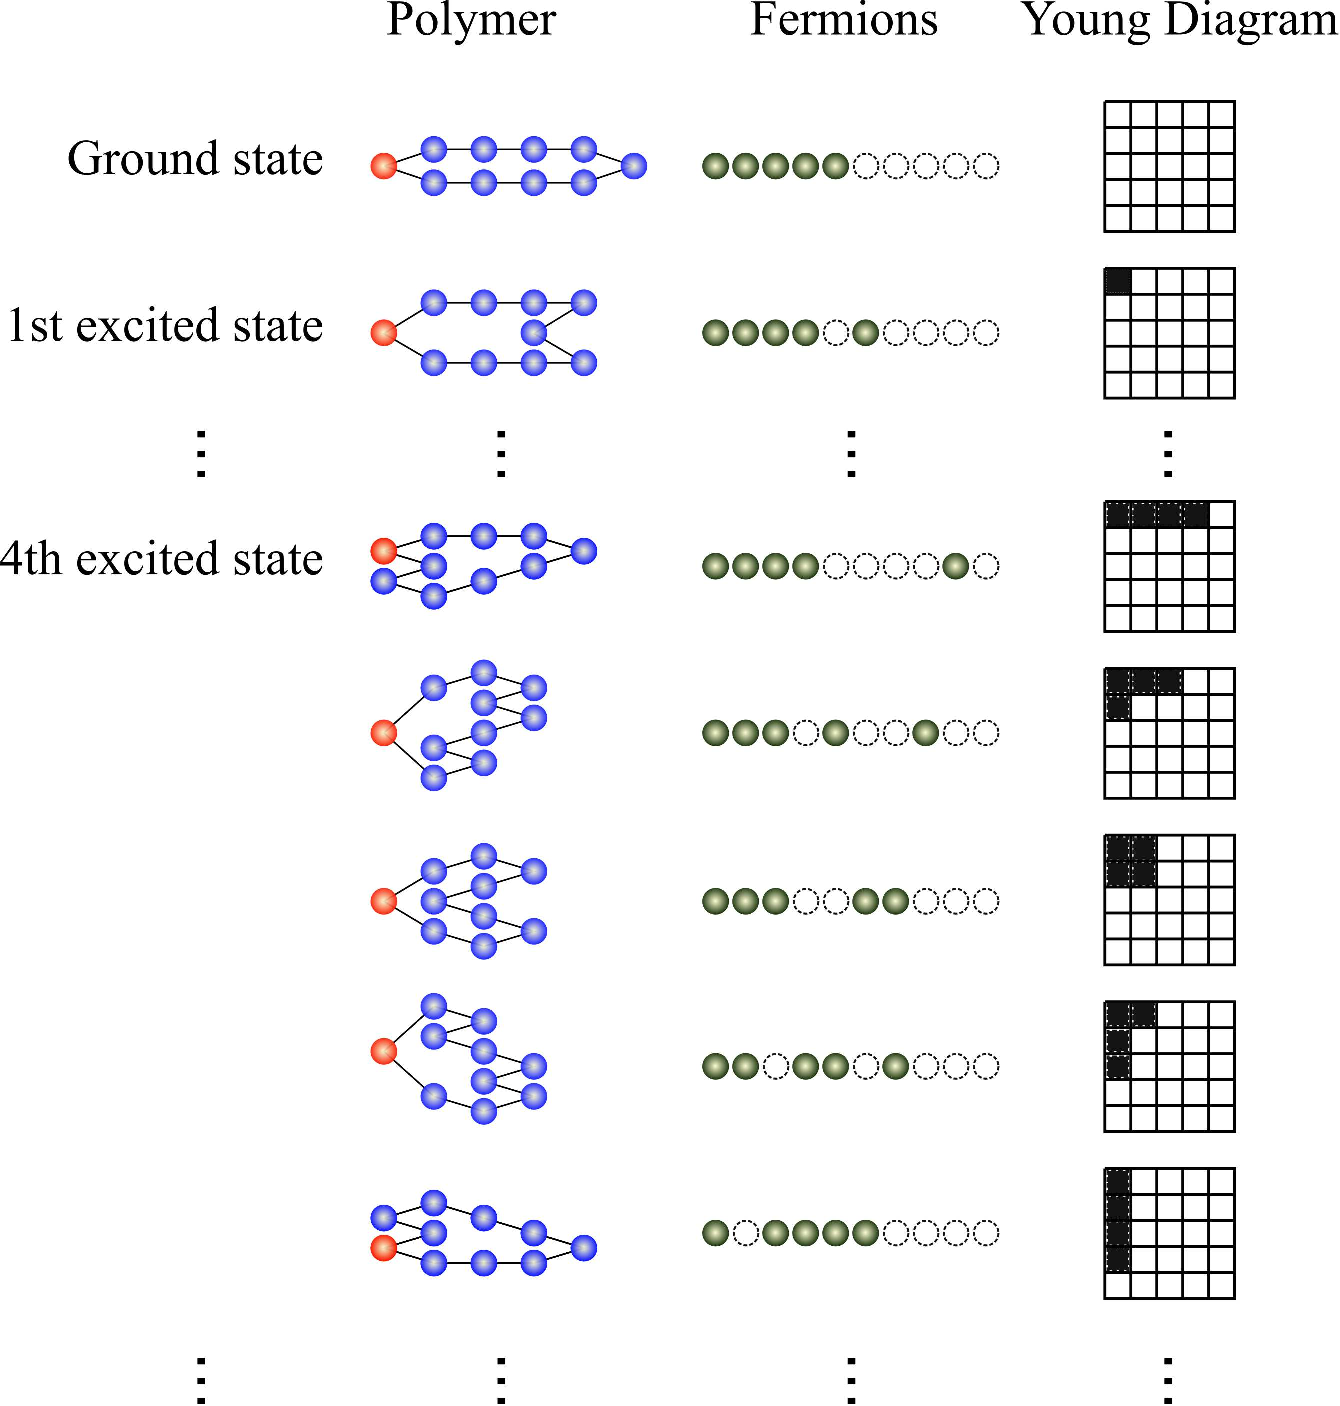
\includegraphics[width=0.45 \textwidth]{schematic}
\caption{Schematic diagram. (a) Polymer blahblihblah (b) Fermion blahblihblah (c) Young diagram didadi...}
\label{fig:schematic}
\end{figure}

\subsection{Number partition theory} 
Although the approach detailed in the above section accurately estimates
the mean and variance of equilibrium position of $j^{\rm th}$ bead, it is an
approximated theory. The random walk is continuous in space and the positions of
the beads resides on an lattice. In addition, the distribution of the position
of any bead in the random-walk picture is always a Gaussian
\cite{Lin2015}, but in the discrete lattice model it is not:
for example, in low temperature, the polymer would be mostly staying in its
fully stretched configuration (see Fig.~\ref{fig:schematic}) and the
distribution of the positions of the beads are always bounded by the natural
length of the rods. 

Analytic solutions are possible in this particular model. We outline the key
ideas in the followings, and leave the more detailed and technical analysis in a
separate article [XXX]. 

Our idea is to change the basis of the Fermionic system from its microscopic
configurations $\left\{Z_0,Z_1,\ldots,Z_{N-1}\right\}$ to the energy of the system.
Clearly, the energy can only take values $E_0, E_0+\Delta E, \ldots, E_0 + N^2
\Delta E / 4$; in this picture, the probability space is a one-dimensional
lattice with finite support. Without lost of generality, we let the constant
energy $E_0=0$ and $\Delta E=1$ by choosing a proper unit. The difficulty of
this basis is to determine the degeneracy of the microscopic states which have
the same energy $E \in \left\{0,1,\ldots N^2/4\right\}$, sometimes referred to as the
``density of the state'' in statistical mechanics \cite{Chandler1987,Huang2001}
and condensed matter physics \cite{Sander2009}. We let the number of
microscopic states with energy $E$ to be $g(E)$; once $g(E)$ is known, the
partition function of the system can be formally derived in the canonical
ensemble picture
\begin{equation}
    \label{partition_func}
    \mathcal{Z}\left(T\right) = \sum_{E=0}^{N^2/4} g(E) \, \exp
    \left(-\frac{E}{k_B T}\right),
\end{equation}
and the equilibrium property of the system can be derived from $\mathcal{Z}$. 

With a little surprise, we discovered that $g(E)$ in this problem is closely
related to the problem of integer partition in number theory
\cite{Andrews1998}. The connection can be made by formulating the problem
in the following way. We consider to label the micro-state of the system by how
many energy unit a Fermion is excited from its ground state. Mathematically, we
denote $E_i$ to be the excited energy of the particle with $i^{\rm th}$ highest
energy. The total energy of the system is
\begin{subequations} 
    \label{eq:partition}
    \begin{align}
        E= \sum_{i=1}^{N} E_i,
    \end{align}
\text{and construction we have a constraint}
    \begin{align}
        \label{eq:partition_constraint}
        N/2 \ge E_1 \ge E_2 \ge \ldots \ge E_{N/2} \ge 0. 
    \end{align}
\end{subequations}
Equations \eqref{eq:partition} constitutes a restricted partition of the integer
$E$: $g(E)$ is the possible ways to partition an integer $E$ into $N/2$
non-increasing parts \cite{Andrews1998}.

A very neat way to label the microscopic configuration is to use the Young
diagram \cite{Andrews1998}, showing in the right panel of Fig.~\ref{fig:schematic}. The
black box in row $i$ denotes the excited energy $E_i$. With the constraint
\eqref{eq:partition_constraint}, each row can have at most $N/2$ black boxes,
and the number of black boxes in $(i+1)^{\rm th}$ row cannot exceed the that in
$i^{\rm th}$ row.  Then, $g(E)$ is the number of possibility of arrangement of
$E$ black boxes onto the $N/2 \times N/2$ ``checkerboard''.

Once the this relation is identified, fruitful results from the number theory
\cite{Andrews1998} can be used to solve our problem. For example, denote  the ways to put
$E$ black boxes onto an $K \times L$ checkerboard with non-increasing number of
black boxes per row by $\pi \left(K,L,E\right)$. A recursive relation exists
\cite{Andrews1998}
\begin{equation}
    \pi\left(K,L,E\right) = \pi\left(K,L-1,E\right) + \pi \left(K-1,L, E-L\right),
\end{equation}
which allows very efficient computations of the
$g(E)=\pi\left(N/2,N/2,E\right)$. In addition, the generating function 
\begin{equation}
    \Phi \left(q\right) := \sum_{E=0}^{N^2/2} g(E) q^E
\end{equation}
is identified to be the Gaussian binomial coefficient
\begin{equation}
    \Phi \left(q\right) \equiv \left(\begin{array}{c} N \\ N/2
        \end{array}\right)_q := \frac{\prod_{j=1}^{N}
        \left(1-q^j\right)}{\left[\prod_{j=1}^{N/2} \left(1-q^j\right)\right]^2},
\end{equation}
which allows us to formulate the partition function of the original polymer
problem \eqref{eq:partition_func}. 
\begin{figure}[htpb]
    \centering
    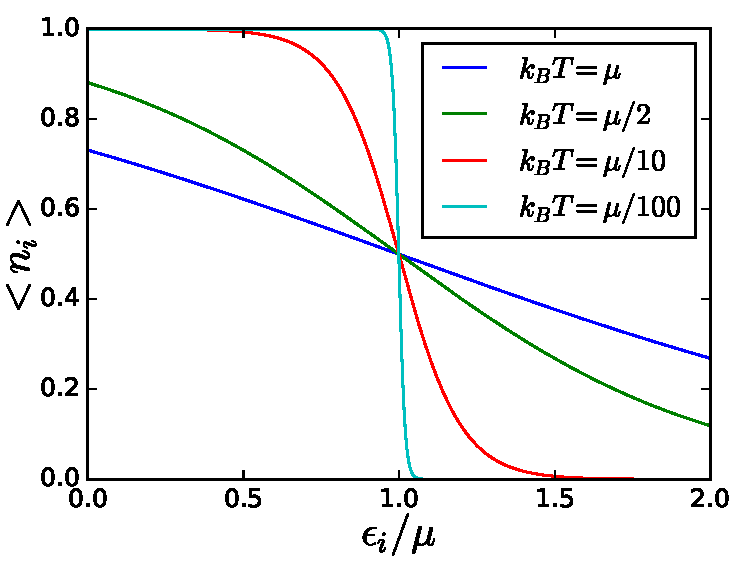
\includegraphics[width=1.0\linewidth]{fermiDrac}
    \caption{Add one figure here about Fermi-Drac distribution}
    \label{fig:fermidrac}
\end{figure}
We finally remark that along this line of analysis, the probability distribution
analogous to \eqref{eq:discrete_prob} can also be formulated. Not surprisingly,
for a finite (and small $N$), the exact results are different from
\eqref{eq:discrete_prob}. With the exact close form partition function, the
mean and variance of bead position can be calculated in the same way of
\eqref{eq:xmean}, this time no ``bridge'' condition is needed. 
Several other physical quantities at equilibrium can
be efficiently computed without resorting to Monte Carlo simulation. We will
present a more detailed analysis separately [XXX].  

\section{Extend the mapping to non-equilibrium}
Having shown the equilibrium statistics been solved by mapping from polymer to
particle, we now come to the discussion about the dynamics. It is intuitively to
extend the analogy to nonequilibrium, i.e., the dynamics of pinned polymer
corresponds to particle diffusion on a one dimensional lattice. To illustrate
the equivalence, we firstly define a typical particle hopping model and build
the connection between these two models. 

\subsection{Asymmetric Exclusion Process}
\label{sec:asep}
As shown in the section above, we consider a 1D lattice with $N$ lattice sites and
exact $N/2$ particles. Only simple exclusive interaction between particle is
applied, and the order of particles is conserved during the particle hopping
process. This is a well studied process named Asymmetric Exclusion Process
(ASEP)\cite{Derrida1998,Schutz2001}. Denote the rate of particle hopping to right and left with
$\alpha$ and $\beta$ respectively, we have the following detailed balance during
the hopping
\begin{equation}
    \alpha P_{n} = \beta P_{n+1} \label{eq:db}
\end{equation}
where $P_{n}$ is the probability of configuration which a particle is sitting
on the $n \rm{th}$ site and ready to hop to right. 
In addition, the ratio of of probability should be proportional to a Boltzmann
factor with the energy difference between these two configurations. Eq
\eqref{eq:db} can be rewrite as 
\begin{equation}
    \beta / \alpha = P_{n} / P_{n+1} = \exp{(-\Delta E / k_B T)}  \label{eq:r_divide_l}
\end{equation}

On the other hand, for a specific particle hopping system, the total hopping
rate is determined by the temperature. External force changes nothing but the
ratio $\alpha/\beta$. Thus we have
\begin{equation}
    \alpha + \beta = r_{total} \label{eq:l_plus_r}
\end{equation}
where $r_{total}$ is a quantity proportional to the temperature $r_{total}
\propto T$. With eq. \eqref{eq:l_plus_r} and eq. \eqref{eq:r_divide_l}
we can in principle solve $\alpha$ and $\beta$ uniquely. The key quantity here is
$\Delta E$, which actually connects polymer and particle model. One can learn
from the polymer and particle equivalence that one particle hopping the right
corresponds to the change of two consecutive rods orientation from right-left to
left-right. Thus the energy difference of the two configuration writes
\begin{equation}
    \Delta E = 2Fa
\end{equation}
Plug into the above equations one obtain
\begin{subequations}
    \label{eq:l_and_r}
    \begin{equation}
        \alpha  =  \frac{r_{total}}{1+\exp{(-2Fa / k_B T)}}
    \end{equation}
    \begin{equation}
        \beta  =   \frac{r_{total}\exp{(-2Fa / k_B T)}}{1+\exp{(-2Fa / k_B
                T)}} \\
    \end{equation}
\end{subequations}
One has to careful to notice that the process of a group of particles hoping to
right is not correspond to the stretching process of the polymer. It is actually
correspond to a spatial motif of polymer configuration moving along the polymer.
Now we have a well defined particle hopping model equivalent to polymer
dynamics in the bulk, but the boundary condition is still not specified. It
turns out the boundary condition together with particle number are crucial to
determinate the type of corresponding polymer.

The pinned polymer loop corresponds to exactly $N/2$ particles hopping on $N$
lattice sites with reflecting boundaries, as discussed in detail for modeling
chromosome in this paper. The mapping can be generalized to other cases, e.g.
un-pinned polymer loop corresponds to $N/2$ particles on $N$ lattice sites with
periodic boundaries, free polymer chain corresponds to an open lattice filled by
arbitrary number of particles. We start and focus on the case of pinned polymer
loop in this paper because of its direct biological relevance. Other cases will
be discussed in our future work.

\subsection{Relaxation Time}
With the ASEP analogy of polymer dynamics, we are ready to go deeper to analyze
the non-equilibrium properties of the polymer system. One of the typical
quantities people interested about dynamics is relaxation time, denote by
$\tau$ here. The protocol here is as following, firstly the trajectories of
particle on ASEP is recorded and then transformed to bead position of polymer
by eq.  \eqref{eq:z2x}, finally relaxation time is fitted from auto-correlation
function (ACF) of interested observables such as gyration radius defined
by $\mathbf{R}_g^2:= \frac{1}{N}\sum_{i=1}^N{\left(\mathbf{r}_i -
        \mathbf{r}_{CM}\right)^2}$.

To get trajectories of hopping particle, we employ the Kinetic Monte Carlo
simulation\cite{Gillespie1976}, which is very fast and efficient compare to Molecular Dynamics
simulation of polymer. By transform to the picture of polymer, we obtain the
dynamical behavior illustrate in Fig. \ref{fig:transient}. 

ACF of gyration radius is calculated based on the information of beads position.
As we see the ACF($Rg$) decays exponentially with time
lag. However, we also observe a effect of multiple relaxation modes indicated
by the beginning part of the curve, especially in the case of strong external
force. This multi-mode behavior is predicted in Rouse model. 
Practically, relaxation time is fitted in the decaying regime where the slope
is most flat, which corresponds to the longest relaxation mode.   
\begin{figure}[htpb]
    \centering
    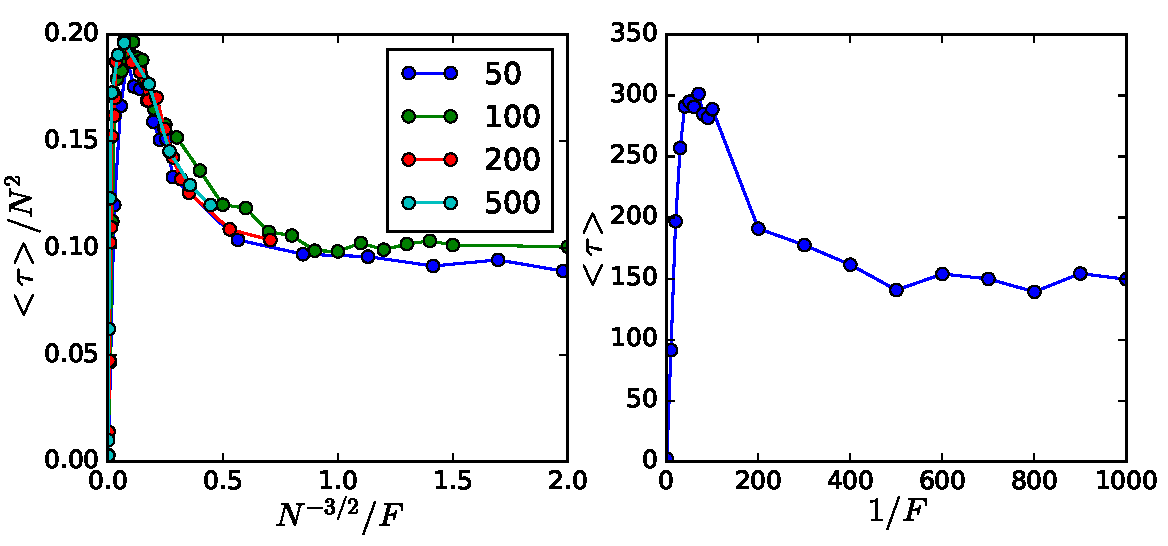
\includegraphics[width=1.0\linewidth]{tauscaling}
    \caption{Relaxation time of gyration radius varies with external force. Left
        1D, right 3D.}
    \label{fig:tauscaling}
\end{figure}
We interested in how the relaxation time varies with the external force field.
So we fixed the temperature $T$ and total hopping rate $r_{total}$ in our model and
simulate the relaxation behavior for different external force. One would
intuitively expect a monotonic decreasing as $F$ grows. Interestingly, we found a
non-monotonic behavior contrast to the expectation, i.e. there is peak which
marks a slowest relaxation time in a weak external force regime. See in Fig.
\ref{fig:relaxation}. To verify the non-monotonic behavior is not artificially
introduced by the reduction of the model, we perform a 3D Brownian dynamics
simulation of pinned bead-rod loop with the same settings. We successfully
reproduced the same behavior of relaxation time varies with external force ---
non-monotonic, as illustrate in Fig. \ref{fig:relaxation}. Moreover,
experimental evidence of this non-monotonic relaxation behavior is also
reported with a similar setting in \cite{Doyle2000}.

A simple theory of relaxation time can be obtained by Rouse
model\cite{Rouse1953,Doi1986}.
However, the rouse model cannot explain the non-monotonic behavior for
relaxation time and external force. In fact, classical Rouse theory predicts the
relaxation time is irrelevant with the external force. The main reason for break
down of Rouse theory is due to the non-extensible rigid rod in our model, in
contrast to the unrealistic infinitely extensible spring in Rouse model. On the
other hand, Rouse theory correctly predicts the scaling law for relaxation time
with system size when external force is not too strong, i.e. $\tau \propto N^2$
when $1/F \gg 1$.

The non-monotonic behavior can be better understood in the corresponding
particle hopping picture. In the strong force case, all particles sit on the
left half of the lattice sites. Only the right-most particle is free to hop
right. In fact, because of the strong hopping bias to the left, even this
particle is not easy to move. Thus a faster relaxation behavior is observed
caused by the strong constraint. On the other hand, when there is totally no
external force applied on the polymer beads, which means there is no bias for
the particle hopping. In this case, the particle will finally evenly
distributed on the lattices sites. The freedom of particle to move is confined
by its neighbors, which is only $2$ lattice sites in average. Since the total
hopping rate is fixed, the relaxation time is proportional to the accessible
distance. In comparison, in the moderate force regime, particle distributed
denser on the left part of lattice and sparser on the right part. The freedom
for those particles on the right side to move is larger than the case of no
external force, and the constraint is not so strong that these particles can
still easily move around. These conditions lead to a longer relaxation time than
the case with no force. 

We now come back to discuss more about the scaling law of relaxation time with
system size. As mentioned above, for relaxation time scales with $N^2$ when
external force is not too strong, predicted by Rouse theory. But how about when
the force is strong? It turns out relaxation time is irrelevant with system size
in this case, i.e. $\tau \propto N^0$. We can again understand this easily
in the particle hopping picture. When the external force is strong, the bias of
particle hopping rate is thus strong. As a result, particles accumulate in the
left side and only few right most particle can move. And the number of movable
particle doesn't depend on the actual total number of particles (polymer size).
In other words, in the case of strong force, only the tail part of the polymer is
fluctuating, the size of this fluctuating blob is not related with the contour
length of the polymer but increase as the external force decrease. Quantitative
results are possible with this understanding and will be discussed in our
future work. Another interesting scaling is how the peak position scales with
the system size. We observe here a scaling of $N^{3/2}$, but lack of physical
understanding of that.

\section{Conclusions}
In conclusion, we demonstrate that 1D polymer can be exactly mapped to a
particle hopping on lattice sites, i.e. ASEP.  We discussed the case of pinned
polymer loop in detail, shown the analytical equilibrium statistics drawing
from the mapping. Furthermore, the dynamics of polymer is also illustrated
in the mapped particle hopping picture. Interestingly, we found that even in
this simple model, there are a lot of non-trivial features such as relaxation
time varies with external force non-monotonically, and different scaling
behavior for relaxation time for different external force. An quantitative
explanation is given by picture of particles hopping on the lattices sites.  

The mapping from polymer to particle is not restricted in the case of pinned
polymer loop. Other generalizations can be investigated with the same mapping,
which leads to ASEP model with different boundaries and particle numbers. We
emphasize the generality of this mapping which can be applied to a huge class of
polymer problems. Moreover, the polymer dynamics beyond 1D is also possible to
model by multi-species ASEP model. There are still a lot of fascinating open
questions to discover in the future.

\begin{acknowledgments}
We would like to acknowledge stimulating discussions with M. Majumdar.
\end{acknowledgments}


% \bibliography{mapping} 
% \bibliographystyle{plain}

\begin{thebibliography}{10}
\bibliographystyle{plain}

\bibitem{Bressloff2013}
Paul~C. Bressloff, Jay~M. Newby, and B.~Derrida.
\newblock {Stochastic models of intracellular transport}.
\newblock {\em Rev. Mod. Phys.}, 301(1-3):135--196, 2013.

\bibitem{Chandler1987}
D~Chandler.
\newblock {\em {Introduction to modern statistical mechanics}}.
\newblock Oxford University Press, 1987.

\bibitem{Chou2011}
T~Chou, K~Mallick, and R~K~P Zia.
\newblock {Non-equilibrium statistical mechanics: from a paradigmatic model to
  biological transport}.
\newblock {\em Reports Prog. Phys.}, 74(11):116601, 2011.

\bibitem{Gennes1981}
Pierre-Gilles de~Gennes.
\newblock {\em {Scaling concepts in polymer physics}}, volume~22.
\newblock Cornell University Press, 1981.

\bibitem{Dekker2013}
Job Dekker, Marc~a Marti-Renom, and Leonid~a Mirny.
\newblock {Exploring the three-dimensional organization of genomes:
  interpreting chromatin interaction data.}
\newblock {\em Nat. Rev. Genet.}, 14(6):390--403, 2013.

\bibitem{Derrida1998}
B.~Derrida.
\newblock {An exactly soluble non-equilibrium system: The asymmetric simple
  exclusion process}.
\newblock {\em Phys. Rep.}, 301(1-3):65--83, 1998.

\bibitem{Ding2004}
DQ~Da~Qiao Ding, Ayumu Yamamoto, Tokuko Haraguchi, and Yasushi Hiraoka.
\newblock {Dynamics of homologous chromosome pairing during meiotic prophase in
  fission yeast}.
\newblock {\em Dev. Cell}, 6(3):329--341, 2004.

\bibitem{Doi1986}
M~Doi and S.f. Edwards.
\newblock {\em {The Theory of polymer dunamics}}.
\newblock Oxford University Press, 1986.

\bibitem{Doyle2000}
P~S Doyle, B~Ladoux, and J~L Viovy.
\newblock {Dynamics of a tethered polymer in shear flow.}
\newblock {\em Phys. Rev. Lett.}, 84(20):4769--4772, 2000.

\bibitem{Gillespie1976}
Daniel~T. Gillespie.
\newblock {A general method for numerically simulating the stochastic time
  evolution of coupled chemical reactions}.
\newblock {\em J. Comput. Phys.}, 22(4):403--434, 1976.

\bibitem{Giorgetti2014}
Luca Giorgetti, Rafael Galupa, Elph{\`{e}}ge~P Nora, Tristan Piolot, France
  Lam, Job Dekker, Guido Tiana, and Edith Heard.
\newblock {Predictive polymer modeling reveals coupled fluctuations in
  chromosome conformation and transcription.}
\newblock {\em Cell}, 157(4):950--63, may 2014.

\bibitem{Halverson2014}
Jonathan~D Halverson, Jan Smrek, Kurt Kremer, and Alexander~Y Grosberg.
\newblock {From a melt of rings to chromosome territories: the role of
  topological constraints in genome folding.}
\newblock {\em Rep. Prog. Phys.}, 77(2):022601, feb 2014.

\bibitem{Huang2001}
Kerson Huang.
\newblock {\em {Statistical Mechanics}}.
\newblock John Wiley {\&} Sons, 2001.

\bibitem{Klebaner2005}
F. C. Klebaner et al.
\newblock {\em {Introduction to stochastic calculus with applications}}.
\newblock World Scientific, 2005.

\bibitem{Sander2009}
L. M. Sander.
\newblock {\em {Advanced condensed matter physics}}, volume~57
\newblock Cambridge University Press, 2009.

\bibitem{Andrews1998}
G. E. Andrews.
\newblock {\em {The theory of partition}}.
\newblock 2.
\newblock Cambridge University Press, 1998.


\bibitem{Lin2015}
Yen~Ting Lin, Daniela Fr{\"{o}}mberg, Wenwen Huang, Petrina Delivani, Mariola
  Chacn, Iva~M. Tolic, Frank J{\"{u}}licher, and Vasily Zaburdaev.
\newblock {Pulled Polymer Loops as a Model for the Alignment of Meiotic
  Chromosomes}.
\newblock {\em Phys. Rev. Lett.}, 115(20):1--8, 2015.

\bibitem{Macdonald1968}
Carolyn~T. MacDonald, Julian~H. Gibbs, and Allen~C. Pipkin.
\newblock {Kinetics of Biopolymerization}.
\newblock {\em Biopolymers}, 6:1--25, 1968.

\bibitem{Rosa2008}
Angelo Rosa and Ralf Everaers.
\newblock {Structure and dynamics of interphase chromosomes.}
\newblock {\em PLoS Comput. Biol.}, 4(8):e1000153, jan 2008.

\bibitem{Rouse1953}
P.~E. Rouse.
\newblock {A Theory of the Linear Viscoelastic Properties of Dilute Solutions
  of Coiling Polymers}.
\newblock {\em J. Chem. Phys.}, 21(7):1272, 1953.

\bibitem{Sachs1995}
R~K Sachs, G~van~den Engh, B~Trask, H~Yokota, and J~E Hearst.
\newblock {A random-walk/giant-loop model for interphase chromosomes.}
\newblock {\em Proc. Natl. Acad. Sci. U. S. A.}, 92(7):2710--4, mar 1995.

\bibitem{Schadschneider2011k}
Andreas Schadschneider, Debashish Chowdhury, and Katsuhiro Nishinari.
\newblock {Modeling of Traffic and Transport Processes}.
\newblock In {\em Stoch. Transp. Complex Syst.}, pages 209--214. 2011.

\bibitem{Vogel2009}
Sven~K Vogel, Nenad Pavin, Nicola Maghelli, Frank J{\"{u}}licher, and Iva~M
  Toli{\'{c}}-N{\o}rrelykke.
\newblock {Self-organization of dynein motors generates meiotic nuclear
  oscillations.}
\newblock {\em PLoS Biol.}, 7(4):e1000087, apr 2009.

\end{thebibliography}

\end{document}
